\documentclass{emulateapj}
\usepackage{graphicx,textcomp,fancyhdr,hyperref}
\begin{document}
\pagestyle{fancy}
\pagenumbering{gobble}
\chead{Summary of \texttt{RadVel} results for TOI-1751 }

% Model comparison table
\begin{deluxetable*}{llrrrrrrr}
\tablecaption{Model Comparison}
\tablehead{\colhead{AICc Qualitative Comparison} & \colhead{Free Parameters} & \colhead{$N_{\rm free}$} & \colhead{$N_{\rm data}$} & \colhead{RMS} & \colhead{$\ln{\mathcal{L}}$} & \colhead{BIC} & \colhead{AICc} & \colhead{$\Delta$AICc}}
\startdata

  AICc Favored Model & $e_{b}$, $K_{b}$, $e_{c}$, $K_{c}$, $\dot{\gamma}$, {$\sigma$}, {$\gamma$} & 11 & 206 & 12.17 & -702.79 & 1449.48 & 1414.24 & 0.00 \\

  \hline \\

  Strongly Disfavored & $e_{c}$, $K_{c}$, $\dot{\gamma}$, {$\sigma$}, {$\gamma$} & 8 & 206 & 12.18 & -711.09 & 1450.11 & 1424.22 & 9.98 \\

  \hline \\

  Ruled Out & $e_{b}$, $K_{b}$, $\dot{\gamma}$, {$\sigma$}, {$\gamma$} & 8 & 206 & 12.33 & -721.71 & 1471.35 & 1445.46 & 31.22 \\

   & $\dot{\gamma}$, {$\sigma$}, {$\gamma$} & 5 & 206 & 12.35 & -729.18 & 1470.30 & 1453.96 & 39.72 \\

\enddata
\label{tab:comp}
\end{deluxetable*}

% Table of best fit parameters
\begin{deluxetable}{lrrr}
\tablecaption{ MCMC Posteriors }
\tablehead{
  \colhead{Parameter} & 
  \colhead{Credible Interval} & 
  \colhead{Maximum Likelihood} & 
  \colhead{Units}
}
\startdata
\sidehead{\bf{Modified MCMC Step Parameters}}

  $P_{b}$ & $\equiv37.468$ & $\equiv37.468$ & days \\

  $T\rm{conj}_{b}$ & $\equiv2458967.95$ & $\equiv2458967.95$ & JD \\

  $T\rm{peri}_{b}$ & $2458969.56^{+0.52}_{-0.77}$ & $2458969.61$ & JD \\

  $e_{b}$ & $0.86^{+0.056}_{-0.048}$ & $0.848$ &  \\

  $\omega_{b}$ & $-2.55^{+0.23}_{-0.22}$ & $-2.55$ & radians \\

  $K_{b}$ & $5.6^{+1.8}_{-1.7}$ & $6.1$ & m s$^{-1}$ \\

  $P_{c}$ & $351.3^{+12.0}_{-8.8}$ & $352$ & days \\

  $T\rm{conj}_{c}$ & $\equiv2458967.95$ & $\equiv2458967.95$ & JD \\

  $T\rm{peri}_{c}$ & $2459060^{+36}_{-74}$ & $2459078$ & JD \\

  $e_{c}$ & $0.17^{+0.16}_{-0.11}$ & $0.15$ &  \\

  $\omega_{c}$ & $-2.61^{+0.58}_{-1.3}$ & $-2.5$ & radians \\

  $K_{c}$ & $4.9^{+0.75}_{-0.71}$ & $5.01$ & m s$^{-1}$ \\

\hline
\sidehead{\bf{Orbital Parameters}}

  $P_{b}$ & $\equiv37.468$ & $\equiv37.468$ & days \\

  $T\rm{conj}_{b}$ & $\equiv2458967.95$ & $\equiv2458967.95$ & JD \\

  $T\rm{peri}_{b}$ & $2458969.56^{+0.52}_{-0.77}$ & $2458969.61$ & JD \\

  $e_{b}$ & $0.86^{+0.056}_{-0.048}$ & $0.848$ &  \\

  $\omega_{b}$ & $-2.55^{+0.23}_{-0.22}$ & $-2.55$ & radians \\

  $K_{b}$ & $5.6^{+1.8}_{-1.7}$ & $6.1$ & m s$^{-1}$ \\

  $P_{c}$ & $351.3^{+12.0}_{-8.8}$ & $352$ & days \\

  $T\rm{conj}_{c}$ & $\equiv2458967.95$ & $\equiv2458967.95$ & JD \\

  $T\rm{peri}_{c}$ & $2459060^{+36}_{-74}$ & $2459078$ & JD \\

  $e_{c}$ & $0.17^{+0.16}_{-0.11}$ & $0.15$ &  \\

  $\omega_{c}$ & $-2.61^{+0.58}_{-1.3}$ & $-2.5$ & radians \\

  $K_{c}$ & $4.9^{+0.75}_{-0.71}$ & $5.01$ & m s$^{-1}$ \\

\hline
\sidehead{\bf{Other Parameters}}

  $\gamma_{\rm hires_j}$ & $3.3^{+1.3}_{-1.4}$ & $3.3$ & m s$-1$ \\

  $\gamma_{\rm apf}$ & $3.9^{+1.8}_{-1.9}$ & $4.0$ & m s$-1$ \\

  $\dot{\gamma}$ & $-0.0036^{+0.0025}_{-0.0024}$ & $-0.0034$ & m s$^{-1}$ d$^{-1}$ \\

  $\ddot{\gamma}$ & $\equiv0.0$ & $\equiv0.0$ & m s$^{-1}$ d$^{-2}$ \\

  $\sigma_{\rm hires_j}$ & $3.7^{+0.52}_{-0.44}$ & $3.32$ & $\rm m\ s^{-1}$ \\

  $\sigma_{\rm apf}$ & $5.96^{+0.79}_{-0.8}$ & $5.75$ & $\rm m\ s^{-1}$ \\

\enddata
\tablenotetext{}{ 74000 links saved}
\tablenotetext{}{
  Reference epoch for $\gamma$,$\dot{\gamma}$,$\ddot{\gamma}$: 2458989.783463 
}
\label{tab:params}
\end{deluxetable}

% Table of derived parameters
\begin{deluxetable}{lrrr}
\tablecaption{ Derived Posteriors }
\tablehead{
  \colhead{Parameter} &
  \colhead{Credible Interval} &
  \colhead{Maximum Likelihood} &
  \colhead{Units}
}
\startdata

\enddata
\end{deluxetable}

% Summary of priors
\begin{deluxetable}{l}
\tablecaption{ Summary of Priors }
\tablehead{}
\startdata

  $K$ constrained to be $>0$\\ \\

  $e_{b}$ constrained to be $<0.99$ \\\\
$e_{c}$ constrained to be $<0.99$ \\ \\

  Bounded prior: $-20.0 < \sigma_{\rm apf} < 20.0$\\ \\

  Bounded prior: $-20.0 < \sigma_{\rm hires_j} < 20.0$\\ \\

\enddata
\end{deluxetable}

% Table of Final Convergence Criterion
\begin{deluxetable}{lrrr}
\tablecaption{ Final Convergence Criterion }
\tablehead{
  \colhead{Criterion} &
  \colhead{Final Value}
}
\startdata

  minAfactor & $ 40.540$ \\

  maxArchange & $  0.019$ \\

  maxGR & $  1.004$ \\

  minTz & $7733.472$ \\

\enddata
\end{deluxetable}

% Table of RV data
\begin{deluxetable}{lrrc}
\tablecaption{ Radial Velocities }
\tablehead{
  \colhead{Time} & 
  \colhead{RV} & 
  \colhead{RV Unc.} & 
  \colhead{Inst.} \\
  \colhead{(JD)} & 
  \colhead{(m s$^{-1}$)} & 
  \colhead{(m s$^{-1}$)} & 
  \colhead{}
}
\startdata

  2458967.95000 & 5.32 & 5.83 & apf \\

  2458967.96400 & -4.34 & 5.50 & apf \\

  2458967.97900 & -2.78 & 5.69 & apf \\

  2459301.94800 & -5.59 & 11.97 & apf \\

  2459315.03600 & 29.01 & 25.31 & apf \\

  2459319.83700 & -15.82 & 13.20 & apf \\

  2459323.01900 & 9.31 & 12.68 & apf \\

  2459328.97500 & -16.53 & 11.70 & apf \\

  2459332.87300 & -32.87 & 21.01 & apf \\

  2459336.96000 & -22.18 & 11.91 & apf \\

  2459342.00300 & 128.06 & 34.47 & apf \\

  2459346.00300 & -9.99 & 14.54 & apf \\

  2459404.85600 & -4.34 & 6.78 & apf \\

  2459414.00400 & -10.45 & 8.64 & apf \\

  2459419.92200 & 15.12 & 6.59 & apf \\

  2459427.88700 & -3.56 & 6.25 & apf \\

  2459465.87100 & -10.57 & 10.89 & apf \\

  2459468.83200 & 9.30 & 8.39 & apf \\

  2459469.79900 & 29.68 & 5.77 & apf \\

  2459470.84200 & 14.41 & 7.53 & apf \\

  2459472.82700 & 14.02 & 6.04 & apf \\

  2459527.06000 & -9.76 & 8.24 & apf \\

  2459542.02300 & 7.08 & 7.20 & apf \\

  2459544.02400 & 13.45 & 6.44 & apf \\

  2459548.00500 & 0.82 & 5.54 & apf \\

  2459551.00200 & 8.65 & 6.51 & apf \\

  2459553.58300 & 5.63 & 6.79 & apf \\

  2459590.88900 & 8.38 & 10.24 & apf \\

  2459592.05600 & 5.35 & 5.72 & apf \\

  2459593.99100 & -5.40 & 5.87 & apf \\

  2459595.05100 & -7.24 & 9.55 & apf \\

  2459595.05100 & -7.24 & 9.55 & apf \\

  2459596.06800 & -17.40 & 28.35 & apf \\

  2459597.04900 & 1.89 & 7.58 & apf \\

  2459597.98100 & 4.22 & 6.46 & apf \\

  2459599.03900 & 3.11 & 6.28 & apf \\

  2459600.06000 & 8.78 & 5.54 & apf \\

  2459600.86300 & 8.47 & 8.27 & apf \\

  2459603.01600 & -3.89 & 5.19 & apf \\

  2459604.94200 & -5.30 & 6.22 & apf \\

  2459606.03600 & 18.22 & 6.33 & apf \\

  2459606.83900 & 0.83 & 6.79 & apf \\

  2459607.84300 & -3.20 & 7.84 & apf \\

  2459610.02400 & -9.64 & 6.16 & apf \\

  2459611.01400 & 11.16 & 7.92 & apf \\

  2459617.89500 & 6.66 & 5.48 & apf \\

  2459618.88600 & 10.47 & 5.75 & apf \\

  2459624.06700 & -1.17 & 5.52 & apf \\

  2459625.04300 & 8.74 & 5.69 & apf \\

  2459631.04900 & -3.10 & 5.83 & apf \\

\tablecomments{ Only the first 50 of 206 RVs are displayed in this table. \
Use \texttt{radvel table -t rv} to save the full \LaTeX\ table as a separate file. }
\enddata
\end{deluxetable}

% Multi-panel figure
 
\begin{figure*}[!h]
\centering 

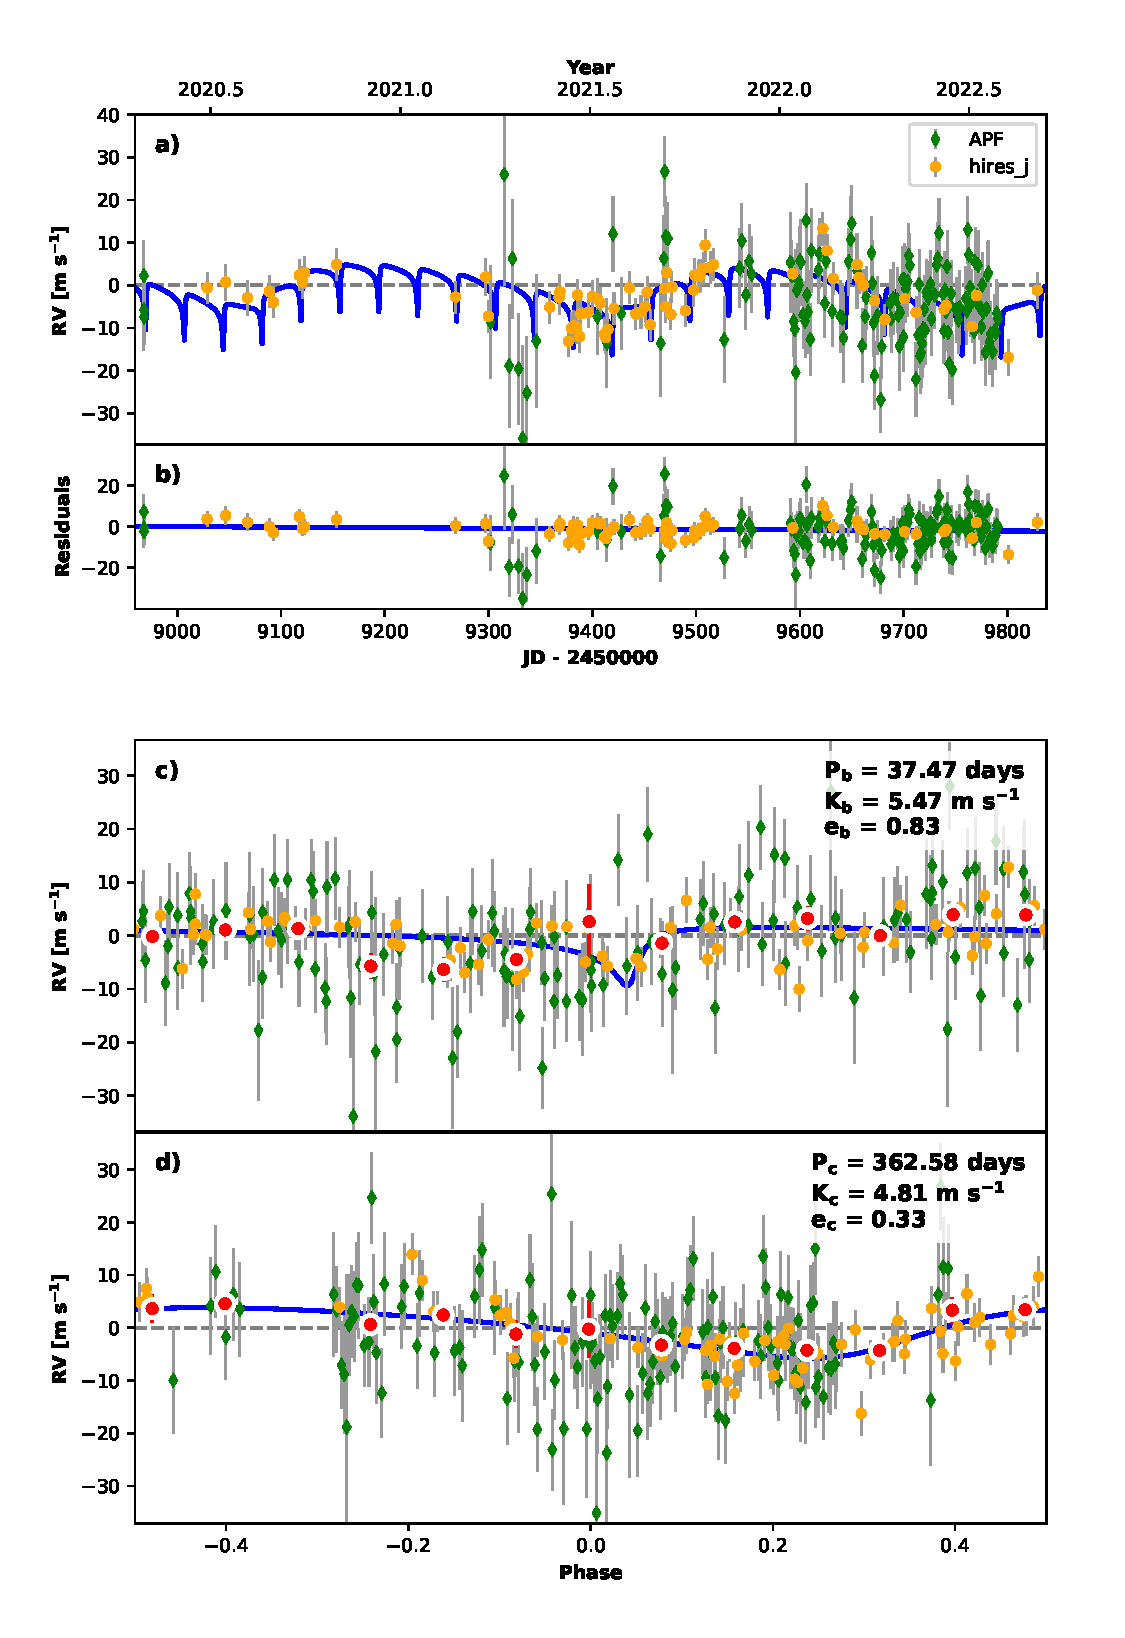
\includegraphics[height=8.0in,width=6.0in,keepaspectratio]{TOI-1751_default_rv_multipanel.pdf}
\caption{ Best-fit 2-planet Keplerian orbital model
  for TOI-1751. The maximum likelihood model is plotted while
  the orbital parameters listed in Table \ref{tab:params} are the
  median values of the posterior distributions.  The thin blue line is
  the best fit 2-planet model. We add in quadrature
  the RV jitter term(s) listed in Table \ref{tab:params} with the
  measurement uncertainties for all RVs.  {\bf b)} Residuals to the
  best fit 2-planet model. {\bf c)} RVs phase-folded
  to the ephemeris of planet b. The Keplerian orbital models for all
  other planets (if any) have been subtracted.  The small point colors
  and symbols are the same as in panel {\bf a}.  Red circles (if
  present) are the same velocities binned in 0.08 units of orbital
  phase.  The phase-folded model for planet b is shown as the blue
  line.}
\end{figure*}
 

% Corner plot
 
\begin{figure*}[!h]
\centering

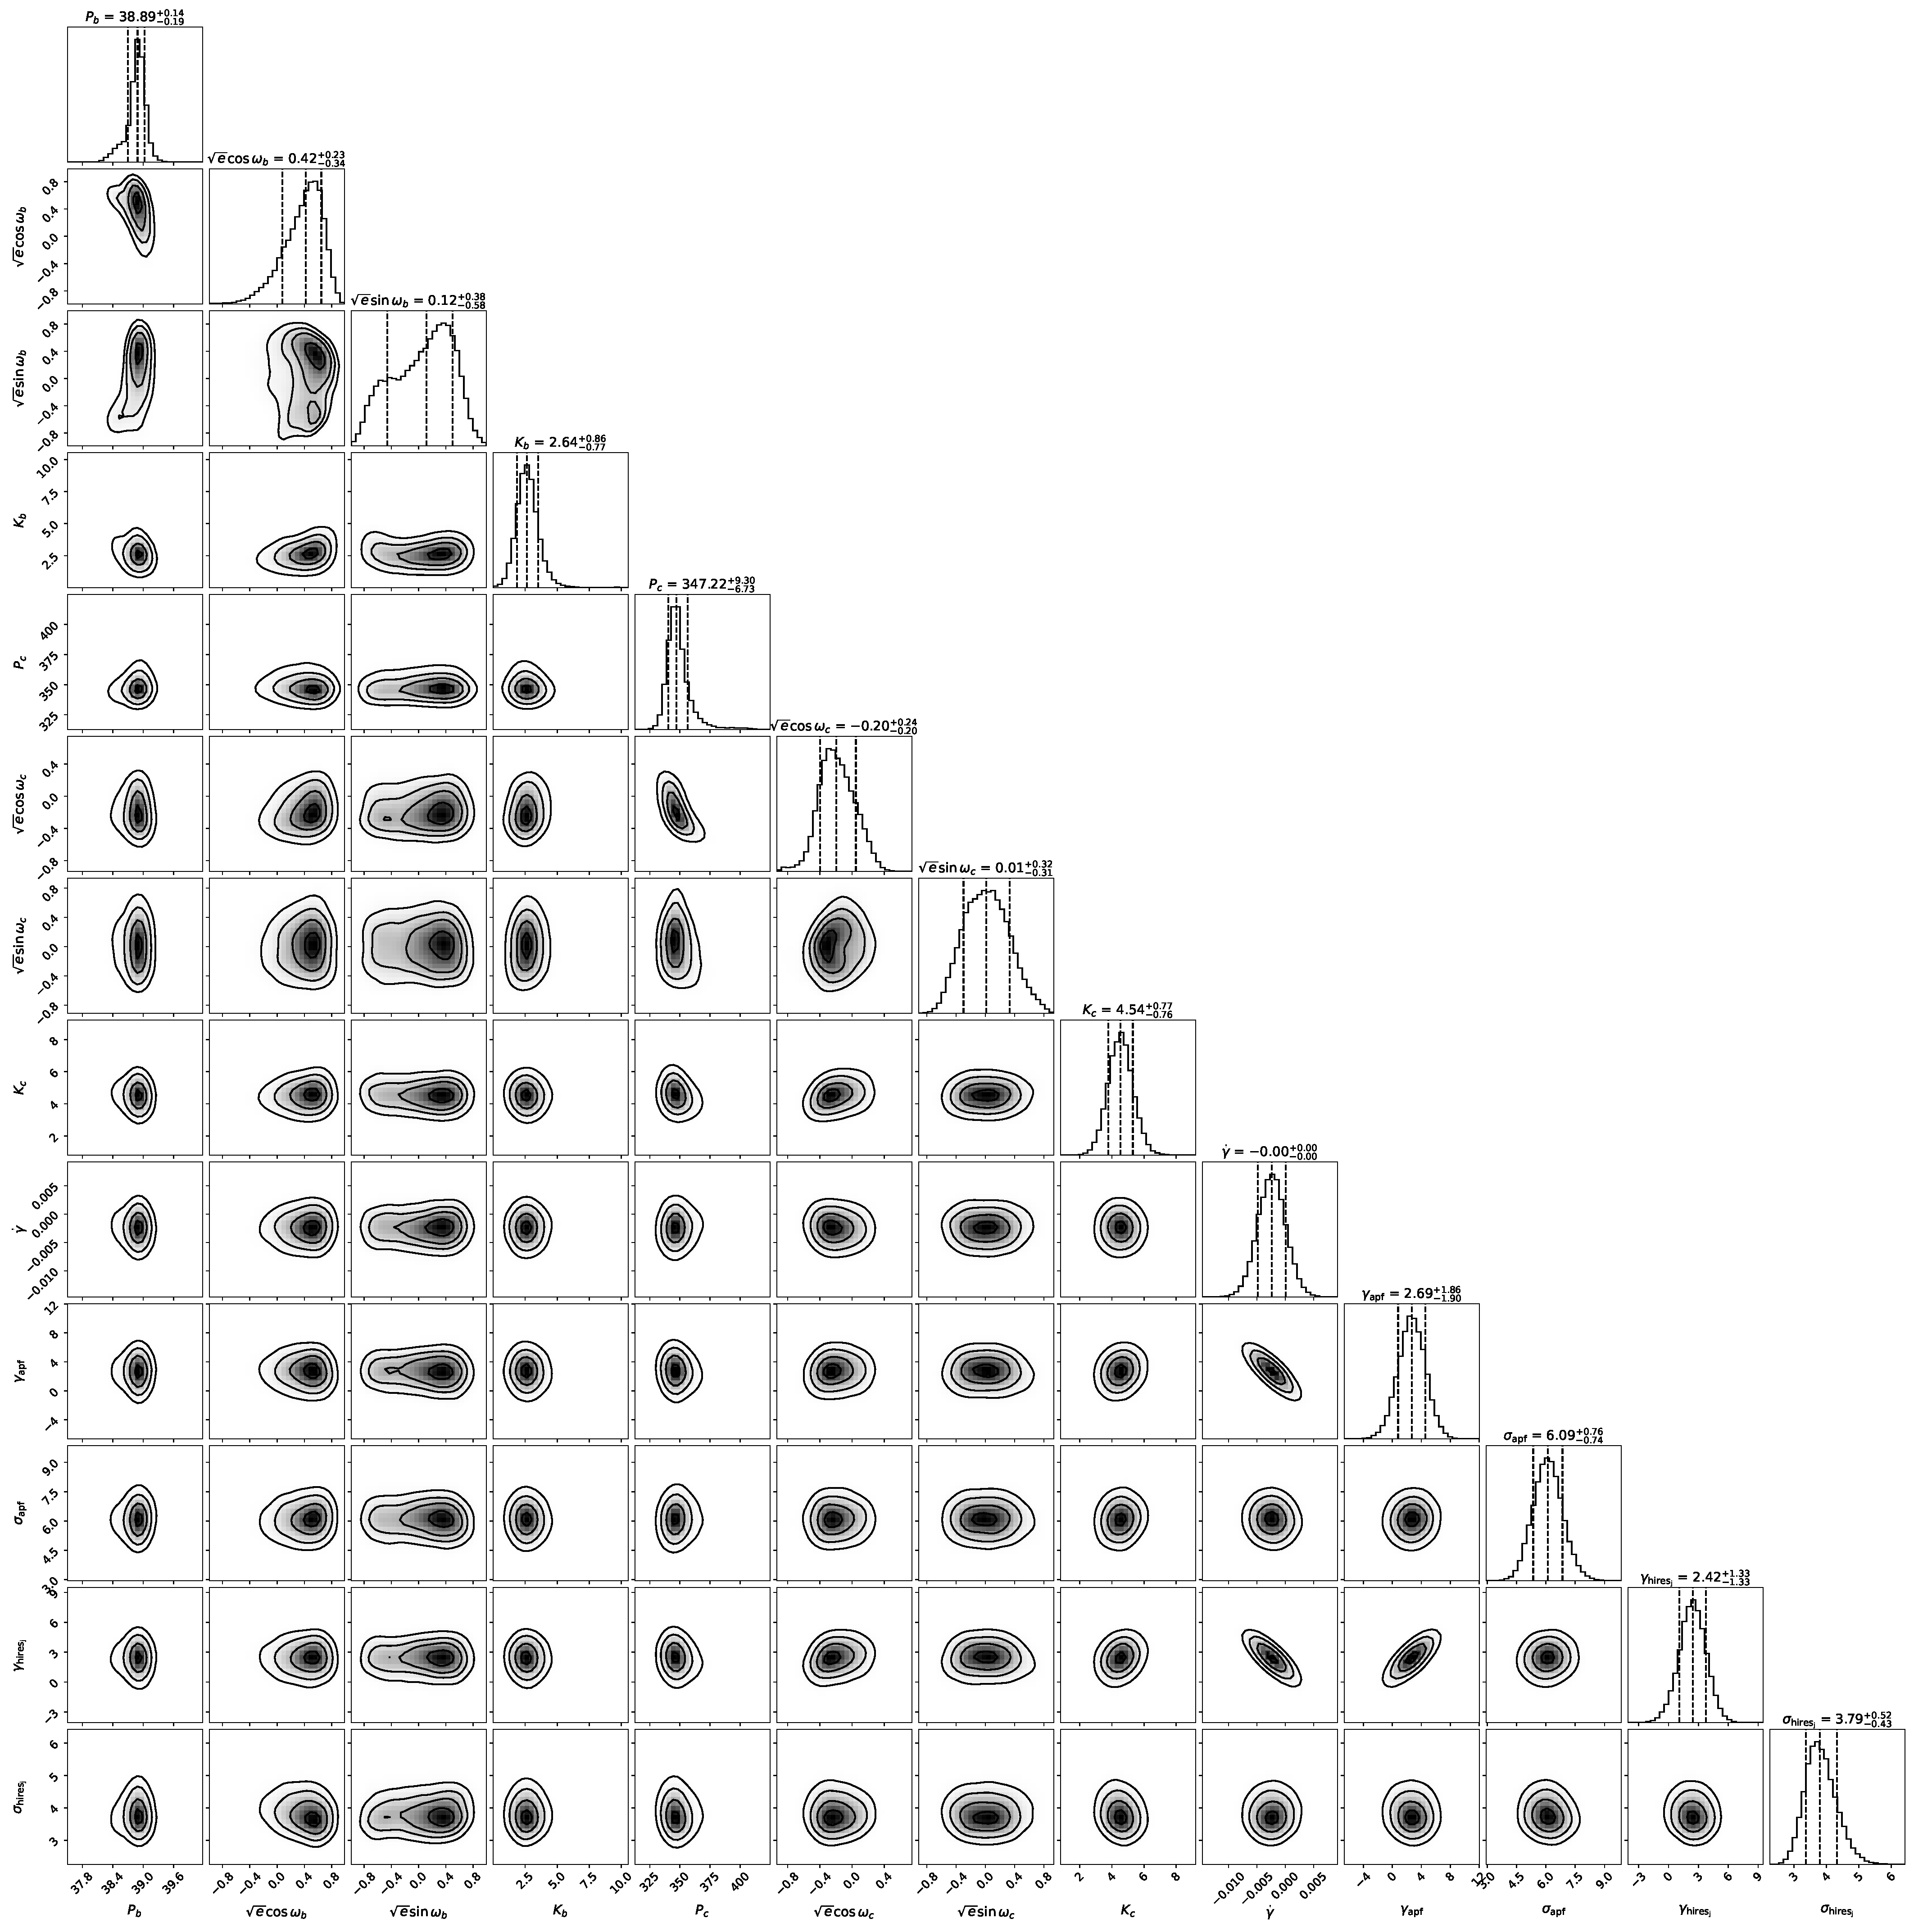
\includegraphics[height=8.0in,width=6.0in,keepaspectratio]{TOI-1751_default_corner.pdf}
\caption{Posterior distributions for all free parameters.}
\end{figure*} 

% Corner plot for derived parameters
 
\begin{figure*}[!h]
\centering

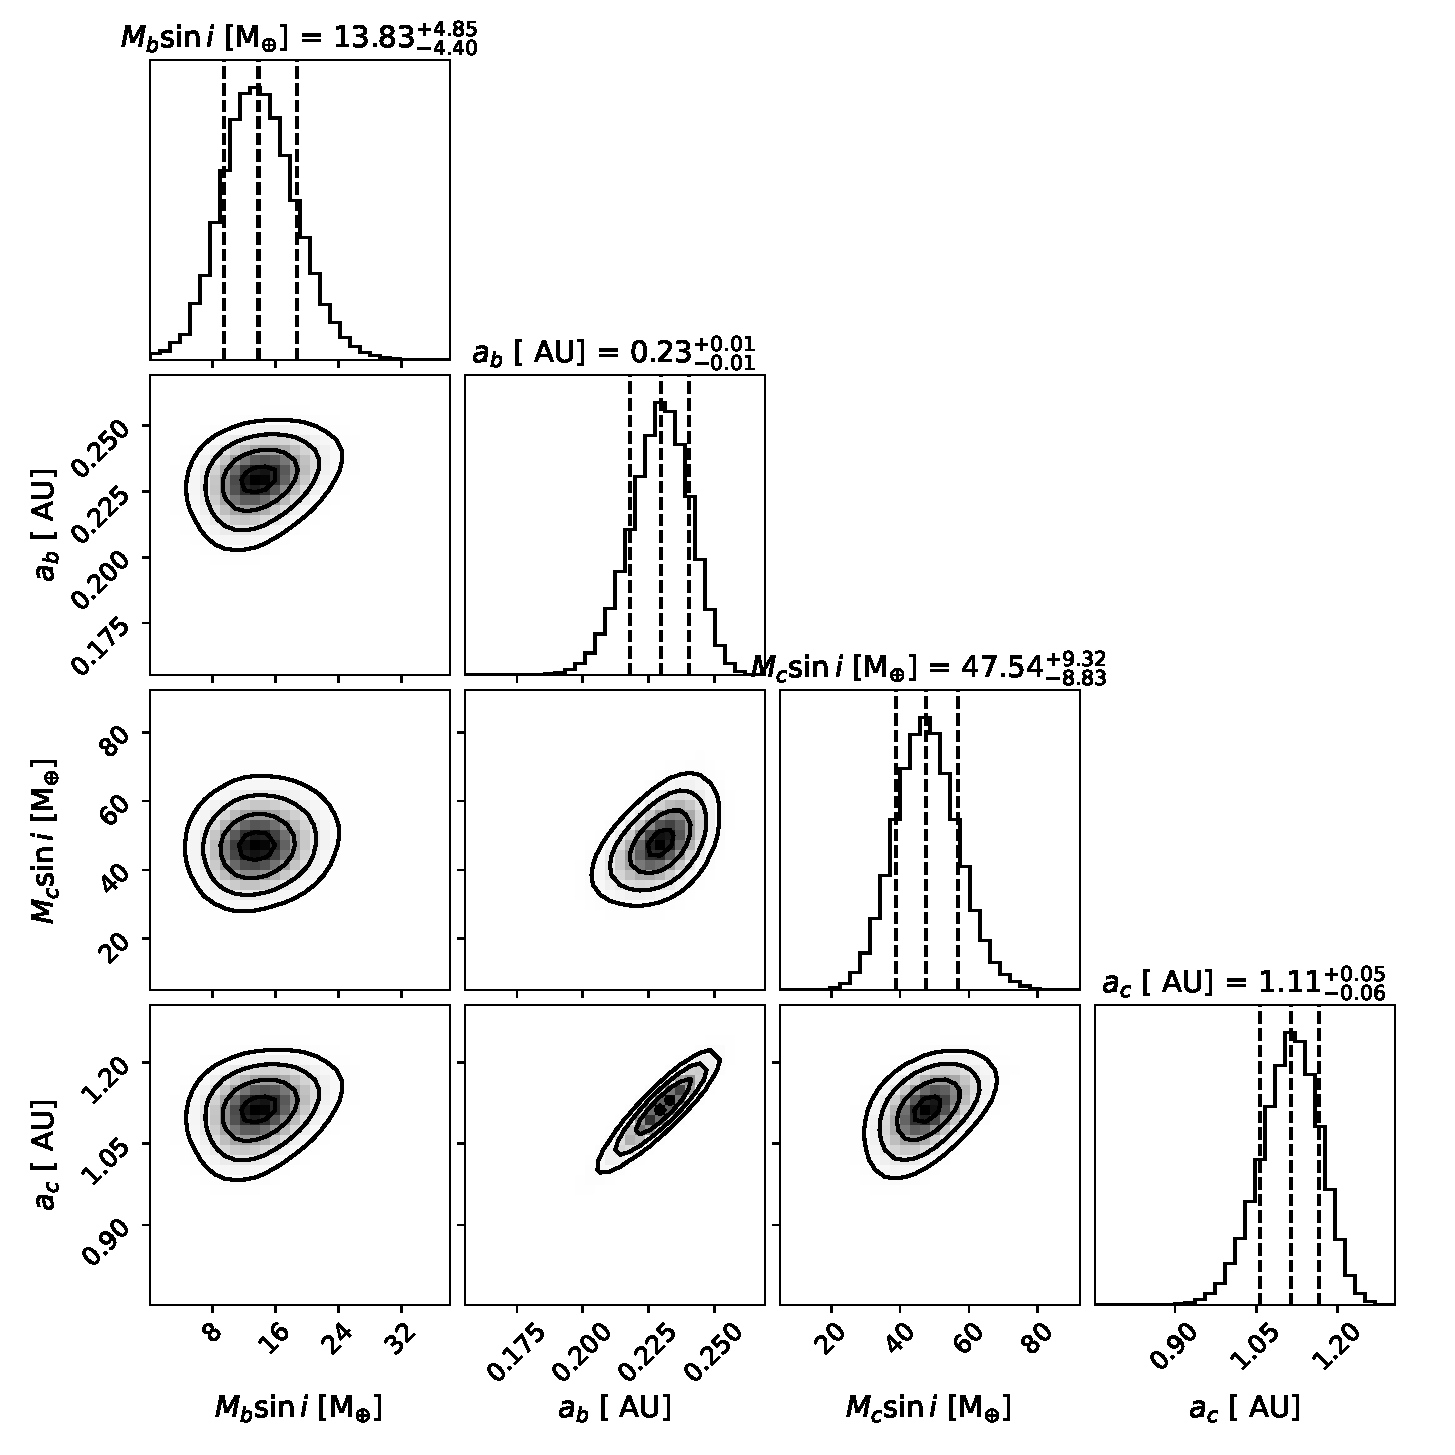
\includegraphics[height=8.0in,width=6.0in,keepaspectratio]{TOI-1751_default_corner_derived_pars.pdf}
\caption{Posterior distributions for all derived parameters.}
\end{figure*} 

\lfoot{
  \footnotesize{
    Report produced by \texttt{RadVel} v1.4.9: 
    \href{http://radvel.readthedocs.io}{http://radvel.readthedocs.io}
  }
}
\end{document}